% Gemini theme
% https://github.com/anishathalye/gemini

\documentclass[final]{beamer}

% ====================
% Packages
% ====================
\usepackage{fontspec}
\usepackage[T1]{fontenc}
\usepackage{lmodern}
\usepackage[size=custom,width=120,height=72,scale=1.0]{beamerposter}
\usetheme{gemini-corners}
\usecolortheme{corners}
\usepackage{graphicx}
\usepackage{booktabs}
\usepackage{tikz}
\usetikzlibrary{arrows.meta}
\usepackage{pgfplots}
\usepackage{multicol}
\setlength{\columnseprule}{1pt}

% ====================
% Lengths
% ====================

% If you have N columns, choose \sepwidth and \colwidth such that
% (N+1)*\sepwidth + N*\colwidth = \paperwidth
\newlength{\sepwidth}
\newlength{\colwidth}
\setlength{\sepwidth}{0.025\paperwidth}
\setlength{\colwidth}{0.3\paperwidth}

\newcommand{\separatorcolumn}{\begin{column}{\sepwidth}\end{column}}

% ====================
% Title
% ====================

\title{Modeling Delay in Multi-hop Networks}

\author{Rachel Wilson \and Pratiksha Thaker \and Justine Sherry}

\institute[shortinst]{Carnegie Mellon University}

% ====================
% Footer (optional)
% ====================

\footercontent{
  \href{mailto:rbwilson@andrew.cmu.edu}{rbwilson@andrew.cmu.edu} \hfill
  Meeting of the Minds, Pittsburgh,
  Spring 2023}
% (can be left out to remove footer)

% ====================
% Logo (optional)
% ====================

% use this to include logos on the left and/or right side of the header:
% \logoright{\includegraphics[height=7cm]{logo1.pdf}}
% \logoleft{\includegraphics[height=7cm]{logo2.pdf}}

% ====================
% Body
% ====================

\begin{document}

\begin{frame}[t]
\begin{columns}[t]
\separatorcolumn

\begin{column}{\colwidth}

  \begin{exampleblock}{Motivation}

    When people send data through a network, they often share bandwidth
    and experience \textit{delay} as queues build on routers.

    \begin{center}
      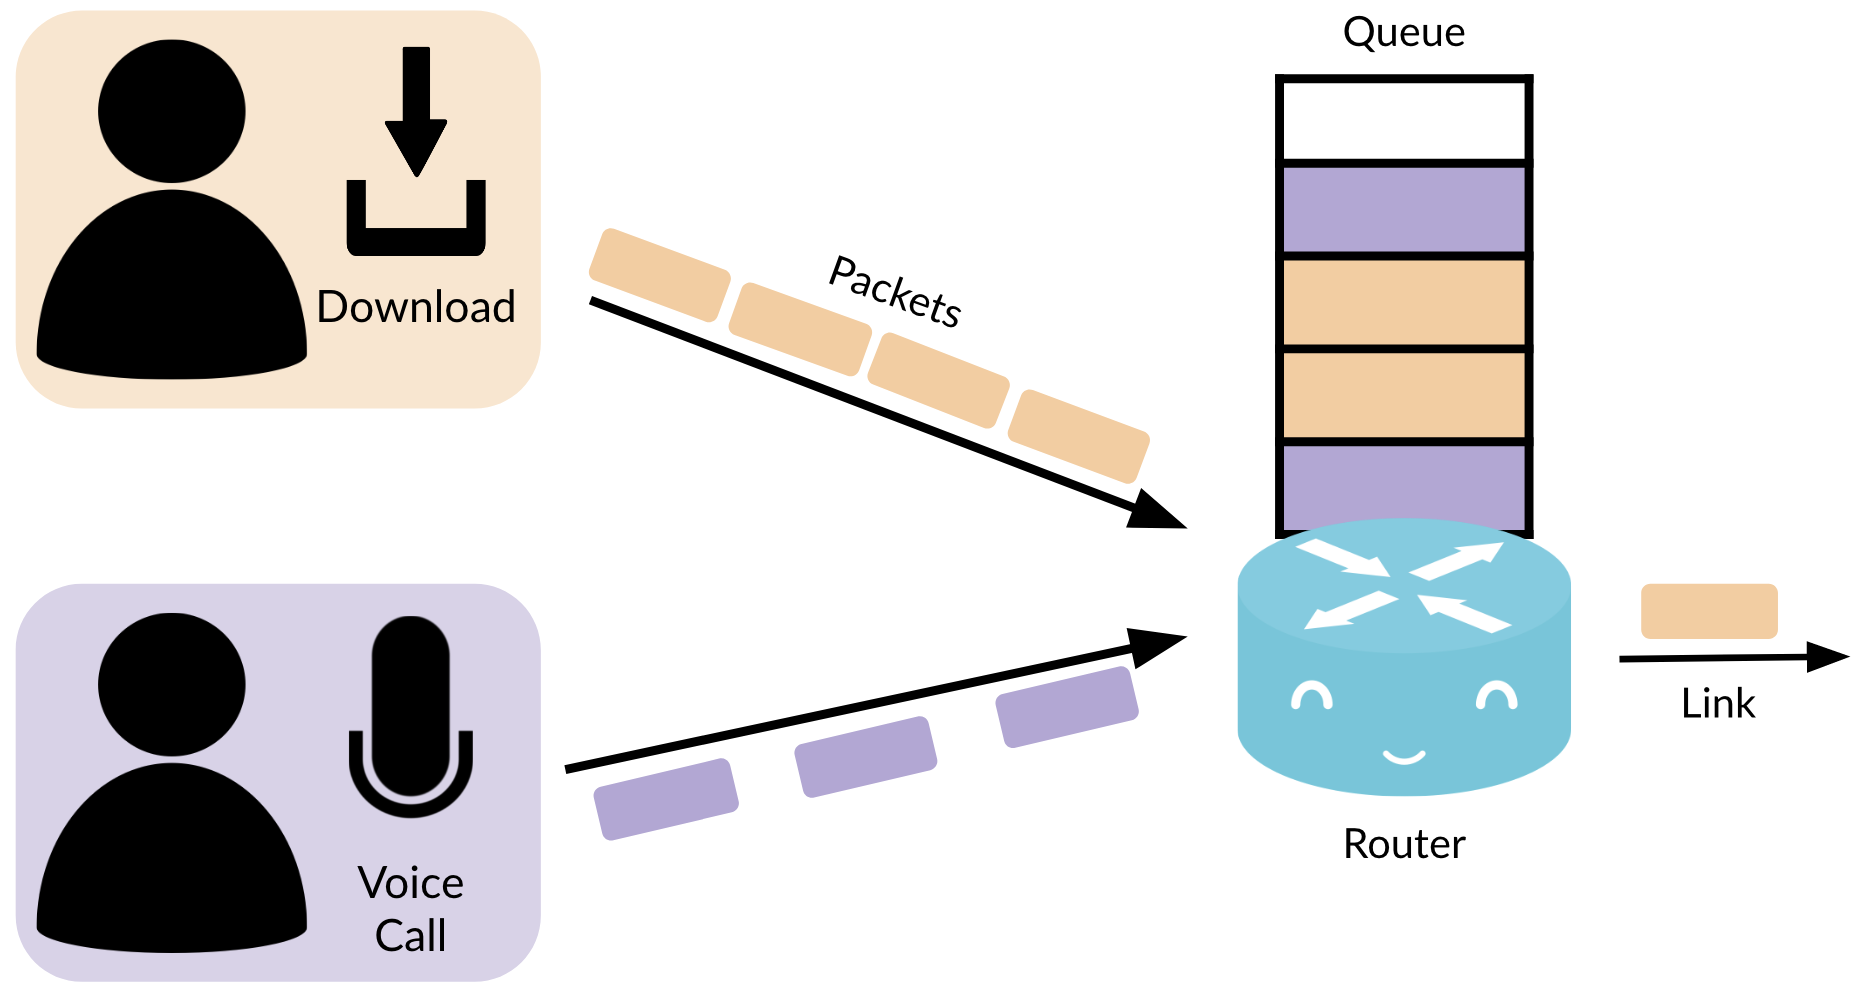
\includegraphics{images/delaydiagram.png}
    \end{center}

    How fast should they send? Too fast and there's delay. Too slow and
    throughput suffers.

    Prior work models this to find optimal sending rates using game theory \cite{hotnets21}.
  \end{exampleblock}

  \begin{block}{Problem}
    \vspace{-5mm}
    Prior work studies multiple senders competing on \textit{one link} \cite{hotnets21}. 
    \textbf{In real networks, senders share multiple links. How can we
    extend this model to multiple senders across multiple links?}
  \end{block}
  \vspace{2mm}

  \begin{alertblock}{Goals}
    \vspace{2mm}
    \begin{enumerate}
      \item \textbf{Model delay for multiple senders}
      \item \textbf{Model delay across multiple links}
      \item \textbf{Model in a way that is simple to integrate with game theory}
    \end{enumerate}
  \end{alertblock}
  \vspace{2mm}

  \begin{block}{Approach}
    \vspace{-5mm}
    First, analyze \textbf{one sender across multiple hops} deterministically.
    
    Next, analyze \textbf{multiple senders across multiple hops} with queueing theory.
  \end{block}
\end{column}

\separatorcolumn

\begin{column}{\colwidth}
  {\LARGE\heading{Delay with One Sender and Multiple Hops}}

  \begin{block}{Setup}
    \vspace{-7mm}
    Links have capacities, $c_i$, that determine its sending speed.
    \begin{center}
      \begin{figure}
        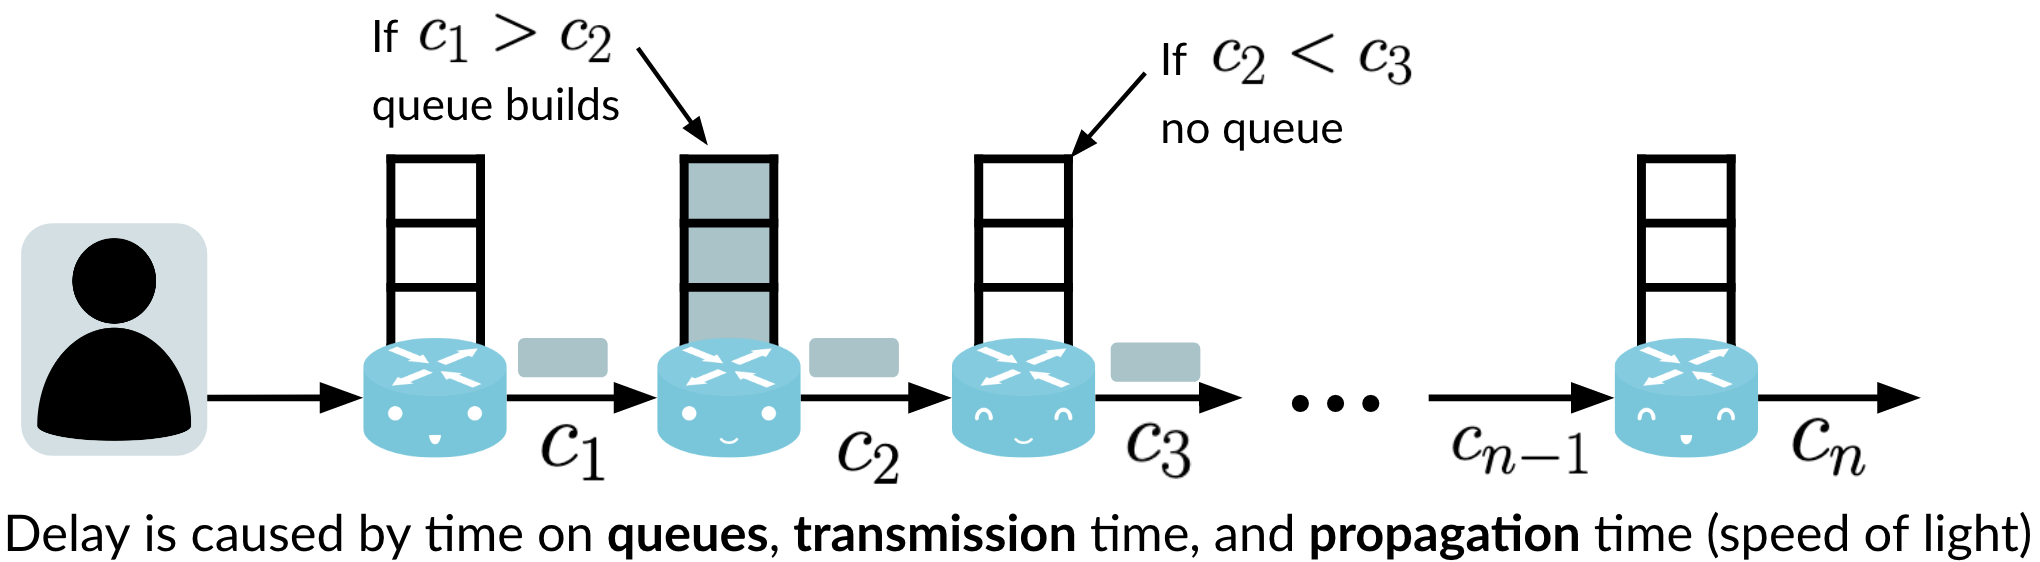
\includegraphics[scale=.9]{images/onesender.png}
      \end{figure}
    \end{center}
    
    How long does it take $p$ packets of $b$ bits each to traverse the network?\\
    It's not obvious how long packets spend on queues.
  \end{block}
  \vspace{-7mm}

  \begin{block}{Result for One Sender}
    \vspace{-7mm}
    Suprisingly, the order of links does not matter. 
    \textbf{End-to-end latency only depends on the slowest link with capacity $c_\mathrm{min}$.}

      \[\mathrm{Total \ time} = \frac{(p-1)b}{c_\mathrm{min}} + \sum_i \frac{b}{c_i}\]
  \end{block}

  \begin{exampleblock}{Proof Sketch}
    \vspace{-7mm}
    \begin{figure}
      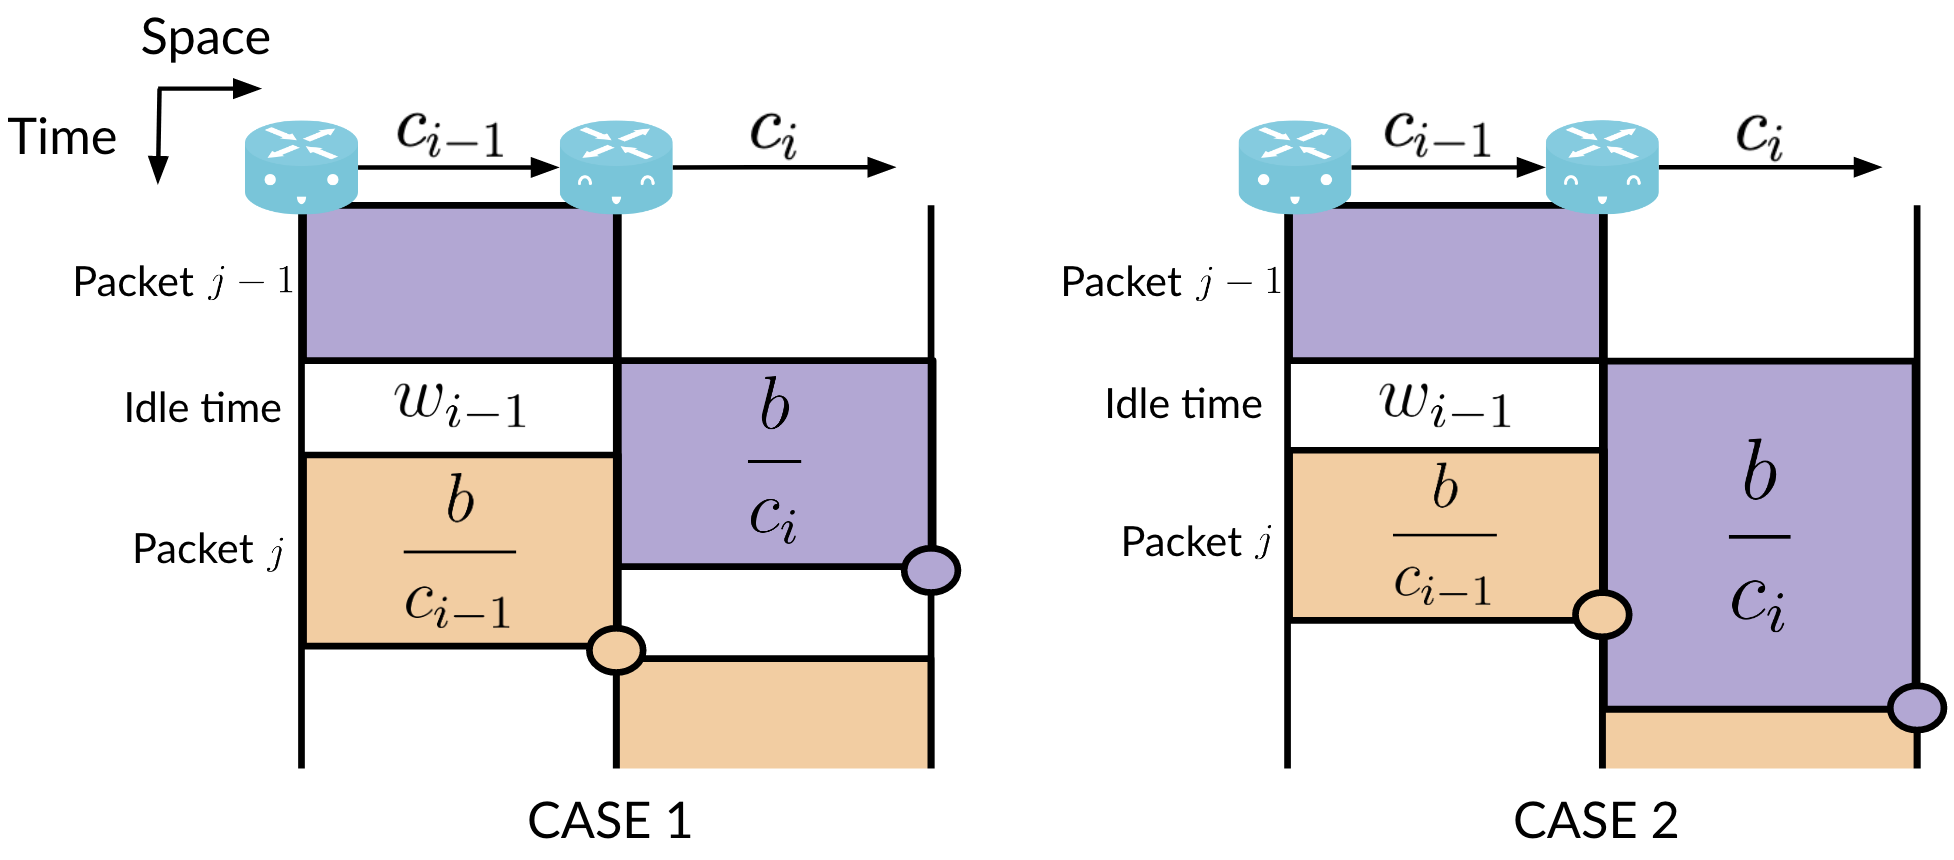
\includegraphics[scale=0.9]{images/spacetime.png}
    \end{figure}
    \vspace{-5mm}
    Between two links, who finishes first? Does time spent per packet change?

    \textbf{Case 1:} {\LARGE$w_{i-1} + \frac{b}{c_{i-1}} \geq \frac{b}{c_i} \to$}
    No change in time between packets

    \textbf{Case 2:} {\LARGE$w_{i-1} + \frac{b}{c_{i-1}} < \frac{b}{c_i} \to$}
    Time increases to the rate of the slower link

    \textbf{Across all links, the time per packet is stretched to the slowest rate.}
  \end{exampleblock}
\end{column}

\separatorcolumn

\begin{column}{\colwidth}
  {\LARGE\heading{Delay with Multiple Senders and Multiple Hops}}

  \begin{block}{Challenge}
    \vspace{-7mm}
    When multiple senders share bandwidth, it's hard to reason deterministically
    about the interleaving of their packets. How do we solve this?
  \end{block}
  \vspace{-6mm}

  \begin{block}{Poisson Processes}
    \vspace{-5mm}
    \begin{center}
      \begin{figure}
        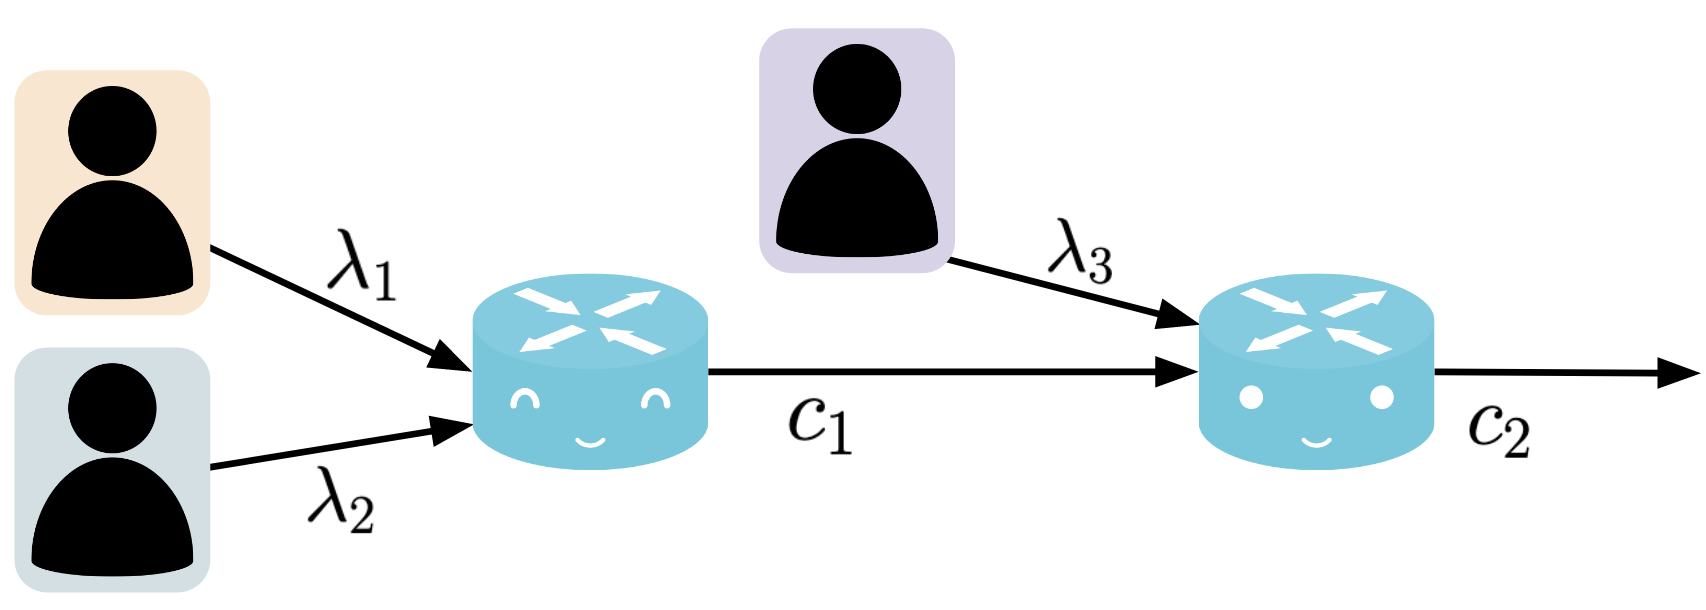
\includegraphics[scale=.65]{images/poisson.png}
      \end{figure}
    \end{center}
    Poisson processes model arrival rates $\lambda$ and link capacities
     $c$. If stable ($\lambda < c$), they have nice properties \cite{morbook}:
     \begin{itemize}
      \item If the input is Poisson($\lambda$), so is the output.
      \item Poisson($\lambda_1$) $+$ Poisson($\lambda_2$) $=$ Poisson($\lambda_1 + \lambda_2$)
     \end{itemize}
  \end{block}
  \vspace{-6mm}

  \begin{block}{Result for Multiple Senders}
    \vspace{-7mm}
    When stable, $\mathbb{E}[T_{\lambda_i}]$ is the average time a packet from $\lambda_i$ spends in the network \cite{morbook}.
    \begin{align*}
      \mathbb{E}[T_{\lambda_1}] = \mathbb{E}[T_{\lambda_2}] &= \frac{1}{c_1 - (\lambda_1+\lambda_2)} + \frac{1}{c_2 - (\lambda_1 + \lambda_2+\lambda_3)}\\
      \mathbb{E}[T_{\lambda_3}] &= \frac{1}{c_2 - (\lambda_1 + \lambda_2+\lambda_3)}
    \end{align*}
  \end{block}
  \vspace{-6mm}

  \begin{block}{Conclusion and Next Steps}
    \vspace{-7mm}
    \textbf{We can now easily model delay for multiple senders over multiple hops.}
    It remains difficult to integrate this into a game theoretic framework.
    
    Towards integration with game theory, we must assess the stability assumption and
    bound the delay so it does not depend on subsets of senders' rates. This will ultimately
    provide minimum throughput guarantees for senders.
  \end{block}
  \vspace{-6mm}

  \begin{block}{References}

    \nocite{*}
    \footnotesize{\bibliographystyle{plain}\bibliography{poster}}

  \end{block}

\end{column}

\separatorcolumn
\end{columns}
\end{frame}

\end{document}
